% --- Motivation ---
\begin{frame}{Evaluation Is the Bottleneck}
  \begin{itemize}\itemsep0.45em
    \item[\textcolor{red}{$\blacktriangleright$}] Every decision in an LLM project is an evaluation decision: which base model to start from, whether a fine-tune helped, whether a prompt change is safe to ship, whether a retrieval pipeline is grounded.
    \item[\textcolor{red}{$\blacktriangleright$}] Training compute is expensive but \textbf{measurable}. Progress is limited by something cheaper and much harder: knowing whether the new system is actually better.
    \item[\textcolor{red}{$\blacktriangleright$}] Generative outputs have \textbf{no single reference answer}. There is no accuracy to compute when the task is ``write a release note'' or ``answer this support ticket from these documents.''
    \item[\textcolor{red}{$\blacktriangleright$}] The consequences of getting this wrong are concrete: a headline benchmark number that does not survive a fresh test set, a leaderboard rank that flips when you reorder the answer options, a judge that prefers whichever answer is longer.
    \item[\textcolor{red}{$\blacktriangleright$}] This lecture is about \textbf{what each measurement actually measures}, and about reporting results honestly enough that someone else could reproduce them.
  \end{itemize}
\end{frame}

\begin{frame}{Benchmarks Have a Shelf Life}
  \begin{columns}[T,onlytextwidth]
    \column{0.46\textwidth}
      \begin{itemize}\footnotesize\itemsep0.4em
        \item[\textcolor{red}{$\blacktriangleright$}] Benchmarks used to last decades. They now \textbf{saturate} within a few years of release: models reach the human reference line, and the benchmark stops separating systems.
        \item[\textcolor{red}{$\blacktriangleright$}] Each curve is normalised so that $-1$ is the first reported result and $0$ is human performance. The slopes get steeper as you move right in time.
        \item[\textcolor{red}{$\blacktriangleright$}] The pattern has continued past this figure: \textbf{GLUE} was superseded by \textbf{SuperGLUE}, \textbf{MMLU} by \textbf{GPQA} and \textbf{Humanity's Last Exam}, \textbf{HumanEval} by \textbf{SWE-bench} and \textbf{LiveCodeBench}.
        \item[\textcolor{red}{$\blacktriangleright$}] Practical consequence: a headline score is only meaningful \textbf{relative to when it was measured} and against which contemporaries.
      \end{itemize}
    \column{0.52\textwidth}
      \centering
      \vspace{0.6em}
      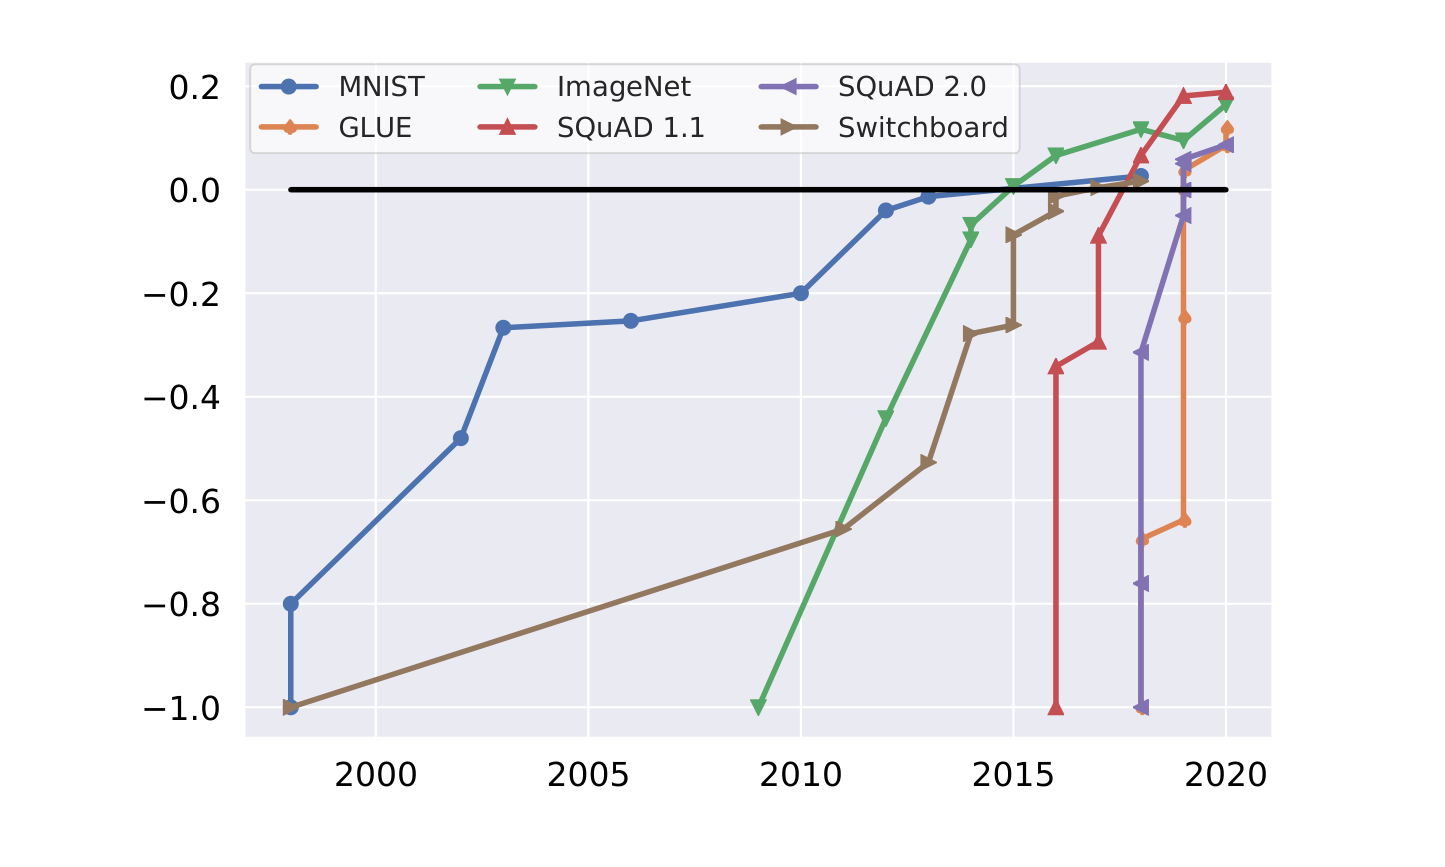
\includegraphics[width=\linewidth,height=0.62\textheight,keepaspectratio]{images/llm-evaluation/dynabench_fig1_benchmark_saturation.png}\\[0.2em]
      {\scriptsize ``Benchmark saturation over time for popular benchmarks, normalized with initial performance at minus one and human performance at zero.'' Kiela et al., ``Dynabench: Rethinking Benchmarking in NLP,'' NAACL 2021, \href{https://arxiv.org/abs/2104.14337v4}{arXiv:2104.14337v4}, Figure 1.}
  \end{columns}
\end{frame}

\begin{frame}{Goodhart's Law and the Optimisation Pressure on Evals}
  \begin{itemize}\itemsep0.4em
    \item[\textcolor{red}{$\blacktriangleright$}] \textbf{Goodhart's law}, in Strathern's compact phrasing: \textit{``When a measure becomes a target, it ceases to be a good measure.''} Benchmarks are targets by construction, so the law applies to all of them.
    \item[\textcolor{red}{$\blacktriangleright$}] The pressure arrives through several distinct channels, and this lecture treats each in turn:
      \begin{itemize}\footnotesize\itemsep0.2em
        \item \textbf{Contamination:} the test set leaks into pretraining, so the score measures memorisation.
        \item \textbf{Format and prompt tuning:} the score measures how well the harness was tuned, not the model.
        \item \textbf{Judge exploitation:} the model learns what an LLM judge rewards --- length, confidence, formatting --- rather than what a user wants.
        \item \textbf{Selection:} report the four benchmarks where you won, quietly drop the six where you did not.
      \end{itemize}
    \item[\textcolor{red}{$\blacktriangleright$}] None of these require bad faith. They are the default outcome of iterating hard against a fixed number.
    \item[\textcolor{red}{$\blacktriangleright$}] The defence is not a better single metric. It is a \textbf{portfolio} of measurements, held-out data you control, and enough statistics to know when a difference is real.
  \end{itemize}
\end{frame}
